\documentclass{exam}
\usepackage[utf8]{inputenc}

\usepackage{mynotes}

\title{Honours Algebra - Week 3 - Abstract Linear Mappings}
\author{Antonio León Villares}
\date{February 2022}

\begin{document}

\maketitle

\tableofcontents

\pagebreak

\textit{Based on the notes by Iain Gordon, Sections 2.3 - 2.4}

\section{Abstract Linear Mappings and Matrices}

\subsection{Generalising Representing Matrices}

\begin{itemize}
    \item \textbf{What is a representing matrix?}
    \begin{itemize}
        \item we found a \textbf{bijection} linking homomorphisms to matrices:
        \[
        M: Hom_\F(\F^m, \F^n) \to Mat(n \times m; \F)
        \]
        \[
        M : f \to [f]
        \]
        \item the bijection was defined by defining a matrix with column vectors as $f(E) \subset \F^n$, where $E$ is the set of standard bases of $\F^m$
    \end{itemize}
    \item \textbf{What is an abstract linear mapping?}
    \begin{itemize}
        \item a linear mapping $f : V \to W$, where $V,W$ are (abstract) vector spaces,\\and $dim(V) = m, dim(W) = n$
        \item we try to relate $V,W$ to $\F^m, \F^n$
    \end{itemize}
    \item \textbf{Can we represent abstract linear mappings as matrices?}
    \begin{itemize}
        \item we know that if $dim V = n$, then there exists an isomorphism between $\F^n$ and $V$, namely:
        \[
        \Phi : \F^n \to V
        \]
        \[
        (\alpha_1, \ldots, \alpha_n) \to \alpha_1\vec{v}_1 + \ldots + \alpha_n\vec{v}_n
        \]
        where $\vec{v}_1, \ldots, \vec{v}_n$ are \textbf{basis vectors} of $V$
        \item it stands to reason from this isomorphism, that linear mappings $V \to W$, with \textbf{ordered bases}, can also be represented via matrices
    \end{itemize}
\end{itemize}

\subsection{Theorem: Abstract Linear Mappings and Matrices}

\textbox{Let $\F$ be a \textbf{field}. 
\\
Let $V,W$ be \textbf{vector spaces} over $\F$, with ordered bases:
\[
A = (\vec{v}_1, \ldots, \vec{v}_m)
\]
\[
B = (\vec{w}_1, \ldots, \vec{w}_n)
\]
respectively.
\\
For each linear mapping:
\[
f : V \to W
\]
we can associate a \textbf{representing matrix of the mapping $f$ with respect to the bases $A$ and $B$}, which we denote as $\cript{f}{B}{A}$.
\\
This is the matrix which turns basis elements in $A$ to an element of $W$, expressed as a linear combination of basis elements in $B$. 
\\
In particular, the entries $a_{ij}$ are given by:
\[
f(\vec{v}_j) = \sum_{i = 1}^n a_{ij}\vec{w}_i, \qquad f(\vec{v}_j) \in W
\]
(since $a_{ij}$ represent the coordinates in the space spanned by $B$).
\\
We again have a bijection (in fact, an \textbf{isomorphism} of vector spaces):
\[
M_B^A: Hom_\F(V, W) \to Mat(n \times m; \F)
\]
\[
M_B^A : f \to \cript{f}{B}{A}
\]
[Theorem 2.3.1]
}

\begin{proof}

Define the isomorphisms:
\[
\Phi_A : \F^m \to V
\]
\[
\Phi_B : \F^n \to W
\]
as at the start of the section. The idea of this proof is summarised in the following diagram:
\begin{figure}[H]
    \centering
    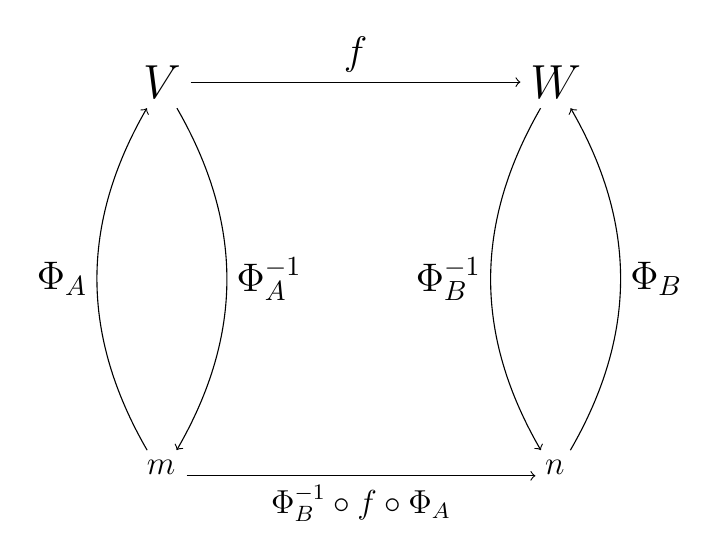
\begin{tikzpicture}
    \node (V) at (0,0) {\LARGE$\boldsymbol{V}$};
    \node (W) at (5,0) {\LARGE$\boldsymbol{W}$};
    \node (Fm) at (0,-5) {\LARGE$\boldsymbol{\F^m}$};
    \node (Fn) at (5,-5) {\LARGE$\boldsymbol{\F^n}$};
    \draw[->] (V) -- (W) node[midway, above] {\Large$f$};
    \draw[->] (Fm) -- (Fn) node[midway, below] {\large$\Phi_B^{-1} \circ f \circ \Phi_A$};
    \draw[->] (Fm) edge[bend left] node[midway, left] {\Large$\Phi_A$} (V);
    \draw[->] (V) edge[bend left] node[midway, right] {\Large$\Phi_A^{-1}$} (Fm);
    \draw[->] (Fn) edge[bend right] node[midway, right] {\Large$\Phi_B$} (W);
    \draw[->] (W) edge[bend right] node[midway, left] {\Large$\Phi_B^{-1}$} (Fn);
    \end{tikzpicture}
\end{figure}

The idea is that we know how to map homomorphisms $\F^m \to \F^n$ to matrices, so if we want a matrix representation of $V \to W$, we can first map it to $\F^m \to \F^n$, and then get the corresponding matrix. To do this:
\begin{enumerate}
    \item map $\F^m$ to $V$ (we have an isomorphism for this)
    \item map $V$ to $W$ (we have $f$ for this)
    \item map $W$ to $\F^n$ (we have an inverse isomorphism for this)
\end{enumerate}
It is then easy to see that we have:
\[
\cript{f}{B}{A} = [\Phi_B^{-1} \circ f \circ \Phi_A]
\]
and the bijection is simply a composition of bijections:
\[
Hom_\F(V,W)  \to Hom_\F(\F^m, \F^n) \to Mat(n \times m; \F)
\]
\[
f \to \Phi_B^{-1} \circ f \circ \Phi_A \to [\Phi_B^{-1} \circ f \circ \Phi_A]
\]

\end{proof}

\sep 

\begin{itemize}
    \item \textbf{How can we represent  mappings from or to the standard bases?}
    \begin{itemize}
        \item the standard basis of $\F^n$ is:
        \[
        S(n)
        \]
        \item whilst we could explicitly write:
        \[
        \cript{f}{S(m)}{S(n)}
        \]
        \[
        \cript{f}{S(m)}{A}
        \]
        \[
        \cript{f}{B}{S(n)}
        \]
        it is more concise to use:
        \[
        [f]
        \]
        \[
        \cript{f}{}{A}
        \]
        \[
        \cript{f}{B}{}
        \]
    \end{itemize}
    \item \textbf{How can we define the inverse of the bijection $\F^n \to V$?}
    \begin{itemize}
        \item let $\Phi_A$ be the bijection:
        \[
        (\alpha_1, \ldots, \alpha_n) \to \alpha_1\vec{v}_1 + \ldots + \alpha_n\vec{v}_n
        \]
        with $A = \{\vec{v}_1, \ldots, \vec{v}_n\}$
        \item the \textbf{inverse} is given by:
        \[
        \Phi_A^{-1} : \vec{v} \to \cript{\vec{v}}{A}{}
        \]
        where $\cript{\vec{v}}{A}{} \in \F^n$ is a \textbf{column vector}
        \item we call $\cript{\vec{v}}{A}{}$ the \textbf{representation of the vector $\vec{v}$ with respect to the basis $A$}, since depending on the basis vectors used by $V$, the elements of $\cript{\vec{v}}{A}{}$ will differ
    \end{itemize}
\end{itemize}

\subsection{Theorem: The Representing Matrix of a Composition of Linear Mappings}

\label{t232}
\textbox{Let $\F$ be a field.
\\
Let $U,V,W$ be \textbf{finite} dimensional vector spaces over $F$, with ordered bases $A,B,C$.
\\
If
\[
f : U \to V
\]
\[
G : V \to W
\]
are \textbf{linear mappings}, then the \textbf{representing matrix} of the composition:
\[
g \circ f : U \to W
\]
is the \textbf{matrix product} of the \textbf{representing matrices} of $f$ and $g$:
\[
\cript{g \circ f}{C}{A} = \cript{g}{C}{B} \circ \cript{g}{B}{A}
\]
[Theorem 2.3.2]
}

\begin{proof}

The proof just relies on unpacking the notation:
\[
\cript{g \circ f}{C}{A} = [\Phi_C^{-1} \circ (g \circ f) \circ \Phi_A]
\]
\begin{align*}
    &\cript{g}{C}{B} \circ \cript{g}{B}{A} \\
    =& [\Phi_C^{-1} \circ g \circ \Phi_B] \circ [\Phi_B^{-1} \circ f \circ \Phi_A] \\
    =& [\Phi_C^{-1} \circ g \circ \Phi_B \circ \Phi_B^{-1} \circ f \circ \Phi_A] \\
    =& [\Phi_C^{-1} \circ (g \circ f) \circ \Phi_A]
\end{align*}

so both sides are equal.

\end{proof}

\subsection{Theorem: Representation of the Image of a Vector}

\textbox{Let $\F$ be a field.
\\
Let $V,W$ be \textbf{finite} dimensional vector spaces over $\F$, with ordered bases $A,B$.
\\
Let
\[
f : V \to W
\]
be a \textbf{linear mapping}.
\\
For $\vec{v} \in V$:
\[
\cript{f(\vec{v})}{B}{} = \cript{f}{B}{A} \circ \cript{\vec{v}}{A}{}
\]
In other words, to get the image of $\cript{\vec{v}}{A}{}$ in the basis $B$ of $W$, we just need to apply the representing matrix with respect to $A$ and $B$. [Theorem 2.3.4]
}

\begin{proof}

As above, we show that both sides are equal:
\[
\cript{f(\vec{v})}{B}{} = \Phi_B^{-1}(f(\vec{v})), \qquad f(\vec{v}) \in W
\]
\begin{align*}
    &\cript{f}{B}{A} \circ \cript{\vec{v}}{A}{} \\
    =& [\Phi_B^{-1} \circ f \circ \Phi_A] \circ \Phi_A^{-1}(\vec{v}) \\
    =& \Phi_B^{-1}(f(\vec{v}))
\end{align*}

\sep 

This can be shown more explicitly. Define:
\[
A = (\vec{v}_1, \ldots, \vec{v}_m)
\]
\[
B = (\vec{w}_1, ºldots, \vec{w}_n)
\]
Define $\cript{f}{B}{A}$ as the $n \times m$ matrix, given by the elements $a_{ij}$ satisfying:
\[
f(\vec{v}_j) = \sum_{ i = 1}^n a_{ij} \vec{w}_i
\]
Since $A$ is a basis of $V$, we can write any $v \in V$ as:
\[
\vec{v} = \sum_{j = 1}^m x_j\vec{v}_j
\]
where $(x_1, \ldots, x_m) \in \F^m$.

\bigskip

Then:
\begin{align*}
    f(\vec{v}) &= \sum_{j = 1}^m x_jf(\vec{v}_j) \\
               &= \sum_{j = 1}^m x_j\left(\sum_{ i = 1}^n a_{ij} \vec{w}_i\right) \\
               &= \sum_{i = 1}^n \left(\sum_{j = 1}^m a_{ij}x_j\right)\vec{w}_i \\
\end{align*}
Notice, we are expressing $f(v)$ using the basis elements of $W$, having started with $\vec{v}$, defined using the basis elements of $V$. If we define:
\[
y_i = \sum_{j = 1}^m a_{ij}x_j
\]
then the whole transformation can be summarised via:
\[
\begin{pmatrix}
y_1 \\
\vdots \\
y_n
\end{pmatrix}
= \cript{f}{B}{A}
\begin{pmatrix}
x_1 \\
\vdots \\
x_m
\end{pmatrix}
\]

\end{proof}

\subsubsection{Examples}
\begin{itemize}
\item recall, in the previous week we define the linear mapping:
\[
f : \mathbb{R}^2 \to \mathbb{R}^2
\]
such that it reflected on the straight line which makes an angle $\alpha$ with the x-axis. If we define $A = (\vec{v}_1, \vec{v}_2)$ with:
\[
\vec{v}_1 = (\cos \alpha, \sin \alpha)^T
\]
\[
\vec{v}_2 = (-\sin \alpha, \cos \alpha)^T
\]
then:
\[
\cript{f}{A}{A} = \begin{pmatrix}
1 & 0 \\
0 & -1
\end{pmatrix}
\]
To see why, it is easier to argue geometrically:
\pic{reflect.png}{0.7}
$\vec{v}_1$ is in the direction of the reflection line (just use the right-angled triangle), so when reflected it won't change. $\vec{v}_2$ is perpendicular to this line, so when reflected, it goes diametrically opposite. In other words:
\[
f(\vec{v}_1) = \vec{v}_1 \qquad f(\vec{v}_2) = -\vec{v}_2
\]
from which the matrix follows (bear in mind $\vec{v}_1 = (1,0)^T, \vec{v}_2 = (0,1)^T$ in the space which they span).

\item consider the following vector spaces:
\[
V = \F_{\leq 3}[x], \qquad A = \{\vec{v}_1 = 1, \vec{v}_2 = x, \vec{v}_3 = x^2, \vec{v}_4 = x^3\}
\]
\[
W = \F_{\leq 2}[x], \qquad B = \{\vec{w}_1 = 1, \vec{w}_2 = 1 + x, \vec{w}_3 = 1 + x^2\}
\]
and define the linear mapping:
\[
D : V \to W
\]
\[
D : v \to \frac{dv}{dx}
\]
We want to find the matrix $\cript{D}{B}{A}$ which performs the mapping $D$, from an eleemnt written via the basis $A$, to an element in $W$ written via the basis $B$. For example, if:
\[
\vec{v} = x^3 = \begin{pmatrix}
0 \\
0 \\
0 \\
1
\end{pmatrix} \in V
\]
Then:
\[
D(x^3) = 3x^2 = 3\vec{w}_3 - 3\vec{w}_1 = \begin{pmatrix}
-3 \\
0 \\
3
\end{pmatrix}\in W
\]
(Technically, the column vector is \textbf{not} part of $V$, but rather of $\F^4$, but it is more useful to think as a column vector, particularly when thinking about $D$ as a matrix)
In other words, we want:
\[
\cript{D}{B}{A} \begin{pmatrix}
0 \\
0 \\
0 \\
1
\end{pmatrix} 
=\begin{pmatrix}
-3 \\
0 \\
3
\end{pmatrix}
\]
We know that:
\[
\cript{D}{B}{A} = [\Phi_B^{-1} \circ D \circ \Phi_A]
\]
Which is nothing but the matrix with column vectors:
\[
\cript{D(\vec{v}_i)}{B}{}
\]
(this is because $\cript{D(\vec{v}_i)}{B}{} = \Phi_B^{-1}(D(\vec{v}_i))$, and as column vectors we want to consider the basis elements)
Hence:
\[
\cript{D(\vec{v}_1)}{B}{} = D(1) = 0 = \begin{pmatrix}
0 \\
0 \\
0 
\end{pmatrix}
\]
\[
\cript{D(\vec{v}_2)}{B}{} = D(x) = 1 = \begin{pmatrix}
1 \\
0 \\
0 
\end{pmatrix}
\]
\[
\cript{D(\vec{v}_3)}{B}{} = D(x^2) = 2x = \begin{pmatrix}
-2 \\
2 \\
0 
\end{pmatrix}
\]
\[
\cript{D(\vec{v}_4)}{B}{} = D(x^3) = 3x^2 = \begin{pmatrix}
-3 \\
0 \\
3 
\end{pmatrix}
\]
Hence, we have that:
\[
\cript{D}{B}{A} = \begin{pmatrix}
0 & 1 & -2 & -3 \\
0 & 0 & 2 & 0 \\
0 & 0 & 0 & 3
\end{pmatrix}
\]
Hence, if  we consider any $\vec{v} = (\alpha, \beta, \mu, \omega)^T \in V$ (again, technically not in $V$), we can convert it to an element of $W$ with basis $B$ using:
\[
\cript{D(\vec{v})}{B} = \cript{D}{B}{A} \cript{\vec{v}}{A}{} \ \implies \ \cript{D(\vec{v})}{B} = \begin{pmatrix}
0 & 1 & -2 & -3 \\
0 & 0 & 2 & 0 \\
0 & 0 & 0 & 3
\end{pmatrix}
\begin{pmatrix}
\alpha \\
\beta \\
\mu \\
\omega
\end{pmatrix}
= \begin{pmatrix}
\beta - 2\mu -3\omega \\
2\mu \\
3\omega 
\end{pmatrix}
\]
We can easily verify that if $\vec{v} = x^3$, this gives the right answer we obtained before. If we then actually want to convert it to an element in $W$ (currently we just have a vector in $\F^3$), we just have to use:
\[
\Phi_B(\cript{D(\vec{v})}{B} ) \ \implies \ \begin{pmatrix}
\vec{w}_1 & \vec{w}_2 & \vec{w}_3
\end{pmatrix}
\begin{pmatrix}
\beta - 2\mu -3\omega \\
2\mu \\
3\omega 
\end{pmatrix}
= (\beta - 2\mu - 3\omega)\vec{w}_1 + 2\mu\vec{w}_2 + 3\omega\vec{w}_3
\]
Notice, if we put this back in terms of the basis $A$, we get:
\[
(\beta - 2\mu - 3\omega)(1) + 2\mu (1 +x) + 3\omega(1+x^2) = \beta + 2\mu x + 3\omega x^2
\]
which is precisely the derivative of:
\[
\alpha + \beta x + \mu x^2 + \omega x^3
\]
as expected.
\end{itemize}

\section{Changing Bases Using Matrices}

\subsection{Theorem: Change of Basis}

\begin{itemize}
    \item \textbf{What is the change of basis matrix?}
    \begin{itemize}
        \item let $V,W$ be vector spaces with respective bases $A,B$
        \item the \textbf{change of basis matrix} is the representing matrix (with respect to $A,B$) defined by the \textbf{identity} mapping:
        \[
        \cript{id_V}{B}{A}
        \]
        \item the entries are given by the $a_{ij}$ satisfying:
        \[
        \vec{v}_j = \sum_{i = 1}^{n} a_{ij}\vec{w}_i, \qquad \vec{v}_j \in A, \vec{w}_i \in B
        \]
    \end{itemize}
\end{itemize}

\sep 

\label{t243}
\textbox{Let $\F$ be a field.
\\
Let $V,W$ be \textbf{finite} dimensional vector spaces over $\F$.
\\
Let:
\[
f: V \to W
\]
be a linear mapping.
\\
Suppose that $V$ has ordered bases $A,A'$.
\\
Similarly, suppose that $W$ has ordered bases $B,B'$.
\\
Then:
\[
\cript{f}{B'}{A'} = \cript{id_W}{B'}{B} \circ \cript{f}{B}{A} \circ \cript{id_V}{A}{A'}
\]
In other words, we can convert the representing matrix with respect to different bases, by applying the change of basis matrix.[Theorem 2.4.3]}

\begin{proof}

From \eqref{t232} we know that:
\[
\cript{g \circ f}{C}{A} = \cript{g}{C}{B} \circ \cript{g}{B}{A}
\]
We also know that:
\[
f = id_W \circ f \circ id_V
\]
(since:
\[
id_W(f(id_V(\vec{v})) = id_W(f(\vec{v}) ) f(\vec{v})
\])
Hence:
\begin{align*}
    &\cript{f}{B'}{A'} \\
    =& \cript{id_W \circ f \circ id_V}{B'}{A'} \\
    =& \cript{id_W \circ (f \circ id_V)}{B'}{A'} \\
    =& \cript{id_W}{B'}{B} \circ \cript{f \circ id_V}{B}{A'} \\
    =& \cript{id_W}{B'}{B} \circ \cript{f}{B}{A} \circ \cript{id_V}{A}{A'} \\
\end{align*}

\end{proof}

\subsubsection{Examples}

As above, define the linear mapping:
\[
f : \mathbb{R}^2 \to \mathbb{R}^2
\]
such that it reflected on the straight line which makes an angle $\alpha$ with the x-axis. Define $B = (\vec{v}_1, \vec{v}_2)$ with:
\[
\vec{v}_1 = (\cos \alpha, \sin \alpha)^T
\]
\[
\vec{v}_2 = (-\sin \alpha, \cos \alpha)^T
\]
and use $A = (\vec{e}_1, \vec{e}_2)$ as the standard basis.
The change of basis matrix has entries satisfying:
\[
\begin{pmatrix}
1 \\
0
\end{pmatrix}
= a_{11}
\begin{pmatrix}
\cos\alpha \\
\sin \alpha
\end{pmatrix}
+
a_{21}
\begin{pmatrix}
-\sin\alpha \\
\cos \alpha
\end{pmatrix}
\]
\[
\begin{pmatrix}
0 \\
1
\end{pmatrix}
= a_{12}
\begin{pmatrix}
\cos\alpha \\
\sin \alpha
\end{pmatrix}
+
a_{22}
\begin{pmatrix}
-\sin\alpha \\
\cos \alpha
\end{pmatrix}
\]
In other words:
\[
\begin{pmatrix}
1 & 0 \\
0 & 1
\end{pmatrix}
= 
\begin{pmatrix}
\cos \alpha & -\sin \alpha \\
\sin \alpha & \cos \alpha
\end{pmatrix}
\begin{pmatrix}
a_{11} & a_{12} \\
a_{21} & a_{22}
\end{pmatrix}
\]
Thus:
\[
\begin{pmatrix}
a_{11} & a_{12} \\
a_{21} & a_{22}
\end{pmatrix}
= 
\begin{pmatrix}
\cos \alpha & -\sin \alpha \\
\sin \alpha & \cos \alpha
\end{pmatrix}^{-1}
\]
since we are just multiplying by the identity matrix.
We know that (yeah, I used the determinant):
\[
\begin{pmatrix}
\cos \alpha & -\sin \alpha \\
\sin \alpha & \cos \alpha
\end{pmatrix}^{-1}
=
\begin{pmatrix}
\cos \alpha & \sin \alpha \\
-\sin \alpha & \cos \alpha
\end{pmatrix}
\]
So then:
\[
\begin{pmatrix}
a_{11} & a_{12} \\
a_{21} & a_{22}
\end{pmatrix}
= 
\begin{pmatrix}
\cos \alpha & \sin \alpha \\
-\sin \alpha & \cos \alpha
\end{pmatrix}
\]

We can then define the change of basis matrix:
\[
\cript{f}{B}{A} = \begin{pmatrix}
\cos \alpha & \sin \alpha \\
-\sin \alpha & \cos \alpha
\end{pmatrix}
\]
What this gives us is a form of converting a vector in $A$ to its corresponding vector in $B$. For example, if we consider:
\[
\cript{\vec{v}_1}{A}{} = (\cos\alpha, \sin\alpha)^T
\]
we know that in terms of the basis $B$, $\cript{\vec{v}_1}{B}{} = (1,0)^T$. Indeed:
\[
\cript{f}{B}{A} \cript{\vec{v}_1}{A}{} = (1,0)^T
\]

\subsection{Corollary: Change of Basis for Endomorphisms}

This is a special case of the Theorem above, whereby instead of using different bases in a different vector space, we consider endomorphisms.

\textbox{Let $V$ be a \textbf{finite} dimensional vector space.
\\
Define the endomorphism:
\[
f : V \to V
\]
Suppose that $A,A'$ are \textbf{ordered bases} of $V$. 
\\
Then:
\[
\cript{f}{A'}{A'} = \cript{id_V}{A}{A'}^{-1} \circ \cript{f}{A}{A} \circ \cript{id_V}{A}{A'}
\]
[Corollary 2.4.4]}

\begin{proof}

It is easy to see that:
\[
\cript{id_V}{A}{A} = \mathbb{I}_n
\]
since, if $\vec{v}_i \in A$:
\[
\vec{v}_i = \sum_{i = 1}^n a_{ij}\vec{v}_i \ \iff \ a_{ij} = \delta_{ij}
\]
Using \eqref{t232}, we know that:
\[
\cript{id_V}{A}{A} = \mathbb{I}_n \ \iff \ \cript{id_V}{A}{A'} \circ \cript{id_V}{A'}{A} = \mathbb{I}_n
\]
Hence, it follows that:
\[
\cript{id_V}{A}{A'}^{-1} = \cript{id_V}{A'}{A}
\]
Thus, if we apply the Theorem above - \eqref{t243} - using $A' = B'$ and $A = B$, we get:    
\[
\cript{f}{A'}{A'} = \cript{id_V}{A'}{A} \circ \cript{f}{A}{A} \circ \cript{id_V}{A}{A'} = \cript{id_V}{A}{A'}^{-1} \circ \cript{f}{A}{A} \circ \cript{id_V}{A}{A'}
\]

\end{proof}

\sep 

\begin{itemize}
    \item \textbf{What are similar matrices?}
    \begin{itemize}
        \item consider:
        \[
        N = \cript{f}{B}{B}
        \]
        \[
        M = \cript{f}{A}{A}
        \]
    \end{itemize}
    \item we say that $N$ and $M$ are \textbf{similar matrices} if:
    \[
    N = T^{-1}MT
    \]
    where:
    \[
    T = \cript{id_V}{A}{B}
    \]
\end{itemize}

\subsubsection{Examples}

Consider $V = \F^2$, and the following bases:
\[
A = \{(1,2)^T, (2,3)^T\} = \{\vec{v}_i\}
\]
\[
B = \{(1,5)^T, (3,2)^T\} = \{\vec{w}_i\}
\]
We want to construct the change of basis matrix:
\[
\cript{id_V}{B}{A}
\]

This matrix has coefficients $a_{ij}$ given by:
\[
\begin{pmatrix}
1 \\
2
\end{pmatrix}
=
a_{11}
\begin{pmatrix}
1 \\
5
\end{pmatrix}
+
a_{21}
\begin{pmatrix}
3 \\
2
\end{pmatrix}
\]
\[
\begin{pmatrix}
2 \\
3
\end{pmatrix}
=
a_{11}
\begin{pmatrix}
1 \\
5
\end{pmatrix}
+
a_{22}
\begin{pmatrix}
3 \\
2
\end{pmatrix}
\]
In matrix form:
\[
\begin{pmatrix}
1 & 2 \\
2 & 3
\end{pmatrix}
= 
\begin{pmatrix}
1 & 3 \\
5 & 2
\end{pmatrix}
\begin{pmatrix}
a_{11} & a_{12} \\
a_{21} & a_{22}
\end{pmatrix}
\]
Notice:
\[
\begin{pmatrix}
1 & 2 \\
2 & 3
\end{pmatrix}
= \cript{id_v}{S(2)}{A}
\]
\[
\begin{pmatrix}
1 & 3 \\
5 & 2
\end{pmatrix}
= \cript{id_v}{S(2)}{B}
\]
To find the change of basis matrix, we just need to invert $\begin{pmatrix}
1 & 3 \\
5 & 2
\end{pmatrix}$:
\[
\begin{pmatrix}
1 & 3 \\
5 & 2
\end{pmatrix}^{-1}
=
-\frac{1}{13}
\begin{pmatrix}
2 & -3 \\
-5 & 1
\end{pmatrix}
\]
So it follows that:
\[
\cript{id_V}{B}{A} = 
-\frac{1}{13}
\begin{pmatrix}
2 & -3 \\
-5 & 1
\end{pmatrix}
\begin{pmatrix}
1 & 2 \\
2 & 3
\end{pmatrix}
=
\frac{1}{13}
\begin{pmatrix}
4 & 5 \\
3 & 7
\end{pmatrix}
\]

\subsubsection{Exercises (TODO)}

\begin{questions}

\question \textbf{Check that Corollary 2.4.4 agrees with the calculations made in the examples above, where we consider the map $f : \mathbb{R}^2 \to \mathbb{R}^2$ to be the reflection on the line through the origin making an angle of $\alpha$ with the x-axis.}

\question \textbf{Let $V$ be an $F$-vector space with ordered basis $A = (\vec{v}_1, \ldots, \vec{v}_n)$. Show that the change of basis matrices lead to a bijection:
\[
\{\text{\textit{ordered bases of $V$}}\} \to GL(n; \F)
\]
\[
B \to \cript{id_V}{B}{A}
\]
where $GL(n; \F)$ is the group of $n \times n$ invertible matrices.
}

To show this is a bijection, it is sufficient to show that it has an inverse, and the inverse is a bijection. In other words, we want a bijection of the form:
\[
GL(n; \F) \to \{\text{\textit{ordered bases of $V$}}\} 
\]
\[
g \to B
\]
We claim that this can be done by using:
\[
B = \{g^{-1}\vec{v}_1, \ldots, g^{-1}\vec{v}_n\}
\]
If we show that:
\begin{itemize}
    \item $B$ is a basis of $V$
    \item $g = \cript{id_V}{B}{A}$
\end{itemize}
then we will have shown that the mapping $g \to B$ is indeed a bijection, and furthermore, an inverse of the original map. To see why this is, its because it allows us to do the following set of mappings:
\[
B \to \cript{id_V}{B}{A} := g \to B
\]
so clearly they are inverses.

\bigskip

We first show that $\{g^{-1}\vec{v}_1, \ldots, g^{-1}\vec{v}_n\}$ is a basis. This is relatively straight forward.

\bigskip

To show linear independence, we can employ the linearity of $g$. Suppose that:
\[
\sum_{i = 1}^n \lambda_i (g^{-1}\vec{v}_i) = 0
\]
Applying $g$, and knowing that as a linear map, $g(0) = 0$:
\[
g\left(\sum_{i = 1}^n \lambda_i (g^{-1}\vec{v}_i)\right) = g(0) \ \implies \ \sum_{i = 1}^n \lambda_i \vec{v}_i = 0
\]
Since $A$ is a basis, we know that $\sum_{i = 1}^n \lambda_i \vec{v}_i = 0$ only when $\lambda_i = 0$, so it follows that the set $B$ s lienarly independent.

\bigskip

Moreover, notice that $V$ is such that $dim(V) = n$. Moreover, $B$ has $n$ elements, so it spans an n-dimensional subspace of $V$. Hence, it follows that $B$ spans $V$. Hence, $B$ must be a basis.

\bigskip

Now, if we compose the mappings, we'd get:
\[
g \to B \to \cript{id_V}{B}{A}
\]
We have a bijection if we have $g = \cript{id_V}{B}{A}$. Now, recall what $\cript{id_V}{B}{A}$ ``means": it is a matrix constructed by being able to write $A = \{\vec{v}_1, \ldots, \vec{v}_n\}$ in terms of $B = \{g^{-1}\vec{v}_1, \ldots, g^{-1}\vec{v}_n\}$ (i.e for each basis element $\vec{v}_i$, we can write it as a linear combination of elements in $B$).

\bigskip

If we consider the inverse mapping:
\[
\cript{id_V}{B}{A}^{-1} = \cript{id_V}{A}{B}
\]
this is the matrix containing the coefficients which allow us to write elements in $B = \{g^{-1}\vec{v}_1, \ldots, g^{-1}\vec{v}_n\}$ in terms of a linear combination of elements in $A = \{\vec{v}_1, \ldots, \vec{v}_n\}$. But clearly, applying  $g^{-1}$ to $\vec{v}_i$ takes us to $g^{-1}\vec{v}_i$. In other words, we must have:
\[
\cript{id_V}{B}{A}^{-1} = \cript{id_V}{A}{B} = g^{-1}
\]
Hence, it must be the case that, as required:
\[
g = \cript{id_V}{B}{A}
\]

\question \textbf{We want to calculate the \textit{order} of the \textit{finite} group $GL(n; \F)$ (recall, the \textit{order} of a group is the number of elements in the group).}

\begin{parts}

\part \textbf{Show that $GL(n;\F_p)$ acts transitively on $\F_p^n \setminus \{0\}\}$. Recall, a \textit{group acts transitively} on a set if for each pair of elements $x,y$ in the set, there is a group element such that $g \cdot x = y$.}

\part \textbf{Determine the stabilizer of the vector $\vec{e}_1 \in \F_p^n$, and establish that:
\[
|Stab_{GL} \ \vec{e}_1| = p ^{n-1}|GL(n-1; \F|
\]
Recall, the \textit{stabiliser} of an element $x$ of a set is a \textit{subgroup} of the group acting on a set. It contains all elements of the group which act on $x$, and do so by mapping it to itself.}

\part \textbf{Using the Orbit Stabilizer Theorem, determine $|GL(n, \F_p)|$. Recall, the \textit{orbit} of an element $x$ is the set of all elements to which the group maps $x$. The orbit stabiliser theorem says that:
\[
|G| = |Stab_G(x)| \times |Orb_G(x)|
\]}

\end{parts}

\end{questions}

\subsection{The Trace}

\begin{itemize}
    \item \textbf{What is the trace of a matrix?}
    \begin{itemize}
        \item the \textbf{trace} of a \textbf{square} matrix is the \textbf{sum} of its \textbf{diagonal} entries
        \item it is denoted using:
        \[
        tr(A)
        \]
        \item in terms of formulae:
        \[
        tr(A) = \sum_{i = 1}n a_{ii}
        \]
    \end{itemize}
    \item \textbf{Are traces defined for infinite rank matrices?}
    \begin{itemize}
        \item only if the sum converges
    \end{itemize}
    \item \textbf{What is the trace of an endomorphism?}
    \begin{itemize}
        \item we can define the \textbf{trace} of an endomorphism:
        \[
        f : V \to V
        \]
        as:
        \[
        tr(f) = tr(f | V) = tr_\F(f | V)
        \]
        \item to compute it, we consider an ordered basis $A$ of $V$, and define:
        \[
        tr(f) = tr(\cript{f}{A}{A})
        \]
        \item turns out, this definition is \textbf{independent} of the basis chosen (reason: $f(AB) = f(BA)$ and $tr(T^{-1}MT) = tr(M)$; this is proven below)
    \end{itemize}
\end{itemize}

\subsubsection{Exercises (TODO)}

\begin{questions}

\question \textbf{Let:
\begin{itemize}
    \item $A$ be an $n \times m$ matrix
    \item $B$ be an $m \times n$ matrix
\end{itemize}
Show that:
\[
tr(AB) = tr(BA)
\]
This is known as the \textit{cyclicity of the trace}.}

\textbox{The above exercise has a very nice implication. In particular, if we pick:
\[
A = T^{-1}M
\]
\[
B = T
\]
then:
\[
tr(T^{-1}MT) = tr(M)
\]
Hence, 2 matrices are similar \textbf{if and only if} they have the same trace.}

\question \textbf{Let $A,B \in Mat(n, \F)$ and $\lambda \in F$.}

\begin{parts}

\part \textbf{Show that:}
\begin{enumerate}
    \item $Tr(\lambda A) = \lambda Tr(A)$
    \item $Tr(A + B) = Tr(A) + Tr(B)$
    \item $Tr(AB) = Tr(BA)$
\end{enumerate}

\part \textbf{Prove that, if:
\[
f : Mat(n; \F) \to F
\]
and:
\begin{itemize}
    \item $f$ is linear (for $f(\lambda A+B) = \lambda f(A) + f(B)$
    \item $f(AB) = f(BA)$
\end{itemize}
then:
\[
f(A) = \alpha Tr(A), \qquad \alpha \in \F
\]
Moreover, show that if $f(\mathbb{I}_n) = n \neq 0$, then:
\[
f(A) = tr(A)
\]
}

The first part is given by dull calculations, so just check \href{https://www.statlect.com/matrix-algebra/trace-of-a-matrix}{this} link with proofs to all the properties (and the exercise above).


\end{parts}

\question \textbf{Let $f : V \to W$ and $g : W \to V$ be 2 linear mappings ($V,W$ are finite dimensional). Show that:
\[
tr(fg) = tr(gf)
\]}

\question \textbf{Let $V$ be finite dimensional, and let $f : V \to V$ be idempotent ($f^2 = f$). Show that:
\[
tr(f) = dim(im(f))
\]}

Last week, in an exercise, we showed that:
\[
ker(\phi \circ \phi) = ker(\phi) \iff V = ker(\phi) \oplus im(\phi)
\]
Since $f$ is idempotent, it must then be the case that:
\[
V = ker(f) \oplus im(f)
\]
Let $\{\vec{k}_1, \ldots, \vec{k}_s\}$ be a basis of $ker(f)$, and let $\{\vec{l}_1, \ldots, \vec{l}_t\}$ be a basis of $im(f)$. Then, a basis of $V$ is given by:
\[
B = \{\vec{k}_1, \ldots, \vec{k}_s, \vec{l}_1, \ldots, \vec{l}_t\}
\]
(This next part I don't understand why)
Hence, the representing matrix, written in block form, will be:
\[
\cript{f}{B}{B} = \begin{pmatrix}
0 & 0 \\
0 & \mathbb{I}
\end{pmatrix}
\]
Thus:
\[
tr(f) = tr(\cript{f}{B}{B}) = dim(im(f))
\]

\question \textbf{Let $V$ be a finite dimensional F-vector space, and $f : V \to V$ a linear mapping. Show that:
\[
tr((f \circ) | End_F(V)) = (dim_FV)tr(f | V)
\]}

\end{questions}

\subsection{Mastering Calculations}

\begin{questions}

\question \textbf{Define a linear map:
\[
f : \mathbb{R}^2 \to \mathbb{R}^2
\]
\[
f(x,y) = (10x - 21y, 4x - 9y)
\]
Let $A$ be the following basis of $\mathbb{R}^2$:
\[
\left(\begin{pmatrix}
2 \\
1
\end{pmatrix},
\begin{pmatrix}
-3 \\
-1
\end{pmatrix}\right)
\]
Determine:
\[
\cript{f}{A}{A}
\]}

\bigskip

We first need to determine where the basis vectors get mapped to under the transformation $f$:
\[
f\left(\begin{pmatrix}
2 \\
1
\end{pmatrix}\right)
=
\begin{pmatrix}
-1 \\
-1
\end{pmatrix}
\]
\[
f\left(\begin{pmatrix}
-3 \\
-1
\end{pmatrix}\right)
=
\begin{pmatrix}
-9 \\
-3
\end{pmatrix}
\]
As we have seen before, the matrix $\cript{f}{A}{A}$ must satisfy:
\[
\begin{pmatrix}
-1 & -9 \\
-1 & -3
\end{pmatrix}
=
\begin{pmatrix}
2 & -3 \\
1 & -1
\end{pmatrix}
\cript{f}{A}{A}
\]
(that is, we can express the basis vectors in $f(A)$ using a linear combination of elements in $A$)
We compute:
\[
\begin{pmatrix}
2 & -3 \\
1 & -1
\end{pmatrix}^{-1}
=
\begin{pmatrix}
-1 & 3 \\
1 & -1
\end{pmatrix}
\]
So:
\[
\cript{f}{A}{A} = 
\begin{pmatrix}
-1 & 3 \\
1 & -1
\end{pmatrix}
\begin{pmatrix}
-1 & -9 \\
-1 & -3
\end{pmatrix}
= 
\begin{pmatrix}
-2 & 0 \\
-1 & 3
\end{pmatrix}
\]

Notice, if we go back to the theorems, we have done nothing else but apply \eqref{t243} (technically Corollary 2.4.4 after):
\[
\cript{f}{A}{A} = \cript{id_{\mathbb{R}^2}}{A}{S(2)} \circ \cript{f}{S(2)}{S(2)} \circ \cript{id_{\mathbb{R}^2}}{A}{S(2)}
\]
where:
\[
\cript{f}{S(2)}{S(2)} = \begin{pmatrix}
10 & -21 \\
4 & -9
\end{pmatrix}
\]
(the matrix corresponding to the linear transformation $f : \mathbb{R}^2 \to \mathbb{R}^2$)
\[
\cript{id_{\mathbb{R}^2}}{S(2)}{A} = \begin{pmatrix}
2 & -3 \\
1 & -1
\end{pmatrix}
\]
(the matrix of the basis elements $A$, in terms of the standard basis)
\[
\cript{id_{\mathbb{R}^2}}{A}{S(2)} = \begin{pmatrix}
-1 & 3 \\
1 & -1
\end{pmatrix}
\]
(the inverse transformation, defining the standard basis in terms of $A$)
Then the computation is automatic:
\[
\cript{f}{A}{A} = \begin{pmatrix}
-1 & 3 \\
1 & -1
\end{pmatrix}
\begin{pmatrix}
10 & -21 \\
4 & -9
\end{pmatrix}
\begin{pmatrix}
2 & -3 \\
1 & -1
\end{pmatrix}
=
\begin{pmatrix}
-2 & 0 \\
-1 & 3
\end{pmatrix}
\]
The other method follows the more intuitive view.

\question \textbf{Let $A$ and $B$ be the following bases of $\mathbb{R}^2$ and $\mathbb{R}^3$ respectively:}
\[
(-2,1)^T, (-3,2)^T
\]
\[
(-2,2,0)^T, (-2,1,0)^T, (4,-2,2)^T
\]
\textbf{The matrix $\cript{f}{B}{A}$ representing the linear mapping:
\[
f : \mathbb{R}^2 \to \mathbb{R}^3
\]
with respect to the bases $A$ and $B$ is the following:
\[
\begin{pmatrix}
-2 & -2 \\
-1 & 1 \\
1 & 2
\end{pmatrix}
\]
Find the matrix which represents the mapping $f$ with respect to the standard bases of $\mathbb{R}^2$ and $\mathbb{R}^3$.} 

We seek $\cript{f}{S(3)}{S(2)}$. By \eqref{t243}, we have:
\[
\cript{f}{S(3)}{S(2)} = \cript{id_{\mathbb{R}^3}}{S(3)}{B} \circ \cript{f}{B}{A} \circ \cript{id_{\mathbb{R}^2}}{A}{S(2)}
\]
Moreover, we have:
\[
 \cript{id_{\mathbb{R}^3}}{S(3)}{B} = \begin{pmatrix}
 -2 & -2 & 4 \\
 2 & 1 & -2 \\
 0 & 0 & 2
 \end{pmatrix}
\]
\[
 \cript{id_{\mathbb{R}^2}}{S(2)}{A} = \begin{pmatrix}
 -2 & -3 \\
 1 & 2 
 \end{pmatrix}
 \ \implies \
  \cript{id_{\mathbb{R}^2}}{A}{S(2)} = \begin{pmatrix}
 -2 & -3 \\
 1 & 2 
 \end{pmatrix}^{-1}
 = 
 \begin{pmatrix}
 -2 & -3 \\
 1 & 2 
 \end{pmatrix}
\]

Thus:
\begin{align*}
    &\cript{f}{S(3)}{S(2)} = \cript{id_{\mathbb{R}^3}}{S(3)}{B} \circ \cript{f}{B}{A} \circ \cript{id_{\mathbb{R}^2}}{A}{S(2)} \\
    \implies \ &\cript{f}{S(3)}{S(2)} = \begin{pmatrix}
 -2 & -2 & 4 \\
 2 & 1 & -2 \\
 0 & 0 & 2
 \end{pmatrix}
\begin{pmatrix}
-2 & -2 \\
-1 & 1 \\
1 & 2
\end{pmatrix}
 \begin{pmatrix}
 -2 & -3 \\
 1 & 2 
 \end{pmatrix}\\
 \implies \ &\cript{f}{S(3)}{S(2)} = \begin{pmatrix}
 -2 & -2 & 4 \\
 2 & 1 & -2 \\
 0 & 0 & 2
 \end{pmatrix}
\begin{pmatrix}
2 & 2 \\
3 & 5 \\
0 & 1
\end{pmatrix}
\\
\implies \ &\cript{f}{S(3)}{S(2)} = 
\begin{pmatrix}
-10 & -10 \\
7 & 7 \\
0 & 2
\end{pmatrix}
\\
\end{align*}

\end{questions}

\end{document}